\documentclass[11pt,onesided]{memoir}

\def\watermarkloaded{0}

\def\Title{ally}
\def\Subtitle{}
\def\FullTitle{\Title}
\def\AuthorFirst{Madison}
\def\AuthorLast{Scott-Clary}
\def\AuthorFull{\AuthorFirst\ \AuthorLast}

\def\Edition{First}
\def\EditionsList{10 9 8 7 6 5 4 3 2 1}
\def\Year{2017}

\def\ISBN{978-1-948743-15-0}

\newenvironment{ally}{
\noindent\ignorespaces
\begin{quotation}
    \allyFont\itshape
    \noindent\ignorespaces}{
\end{quotation}\ignorespacesafterend }

%

%

%%% Resets
% memoir defines footruleskip, we want fancyhdr's
\let\footruleskip\undefined
\DisemulatePackage{setspace}

%%% Hyperref warning suppression
% I want math symbols, hyperref complains
% must be before hyperref included
\usepackage{silence}
\WarningFilter[pdftoc]{hyperref}{Token not allowed in a PDF string}
\ActivateWarningFilters[pdftoc]

%%% Package imports not needing expansion
\usepackage{graphicx}
\usepackage{hyperref}
\usepackage{setspace}
\usepackage{xifthen}
\usepackage{xltxtra}
\usepackage{verse}
\usepackage{paracol}

% page sizes for trade paperback
% 8.5x8.5 + bleed of 0.125 per edge minus spine.
% See https://www.ingramspark.com/hubfs/downloads/file-creation-guide.pdf page 10
\usepackage[
  paperwidth=8.625in,
  paperheight=8.75in,
  layoutwidth=8.625in,
  layoutheight=8.75in,
  vmargin=0.625in,
  outer=0.625in,
  inner=1in,
  includeheadfoot,
  twoside
]{geometry}
\ifdefined\SetWatermarkHorCenter
  \SetWatermarkHorCenter{3in}
  \SetWatermarkVerCenter{4.5in}
\fi


%%% ToC munging
% Remove ToC header
\renewcommand{\contentsname}{}
\renewcommand{\cftdot}{\small{$\cdot$}}
\renewcommand{\cftchapterdotsep}{3}
\renewcommand{\cftsectiondotsep}{10000}
% start toc at top of page
\renewcommand*\tocheadstart{}{}

%%% Font
% Uncomment and modify to your font specs

\usepackage{fontspec}
\setmainfont{Gentium Book Basic}
\newfontface\allyFont{Merriweather Sans Italic}
\newfontfamily\TitleFamily{Inknut Antiqua}
\newfontface\TitleFont{Inknut Antiqua}
% \newfontfamily\DisplayFamily{Playfair Display}
% \newfontface\DisplayFont{Playfair Display}

%%% Headers and page styles
\usepackage[pagestyles]{titlesec}
\usepackage{fancyhdr}
\setlength{\headheight}{15.2pt}

% ourbook style with fancy headers and chapter headings
\fancypagestyle{ourbook}{
  % headers
  \fancyhf{}
  \fancyhf[FRO,FLE]{\thepage}
  % \fancyhf[HLE]{\chaptertitle}
  % \fancyhf[HRO]{\AuthorFull}
  % \renewcommand{\headrulewidth}{0.5pt}
  \setlength{\parskip}{0pt}
  % \parindent0pt
  \setlength{\headheight}{0pt}
}

% plain style with only page num
\fancypagestyle{plain}{
  \fancyhf{}
  \renewcommand{\headrulewidth}{0pt}
  \renewcommand{\footrulewidth}{0pt}
  \fancyhf[FRO,FLE]{\thepage}
}

% single space after periods
\frenchspacing

% Attempt justification at all costs
\sloppy

% Widows and orphans
\widowpenalty=10000
\clubpenalty=10000

%%% Title page
\title{\FullTitle}
\author{\AuthorFull}
\date{}

%%% Section divider
% don't forget to \noindent the line after!
\renewcommand\rule[2]{$\star$}
\newcommand\secdiv{
  \begin{center}
    \rule{}{}
  \end{center}
}

\hyphenation{
\AuthorFirst
\AuthorLast
\Title
\Subtitle
}


\begin{document}
  \frontmatter

  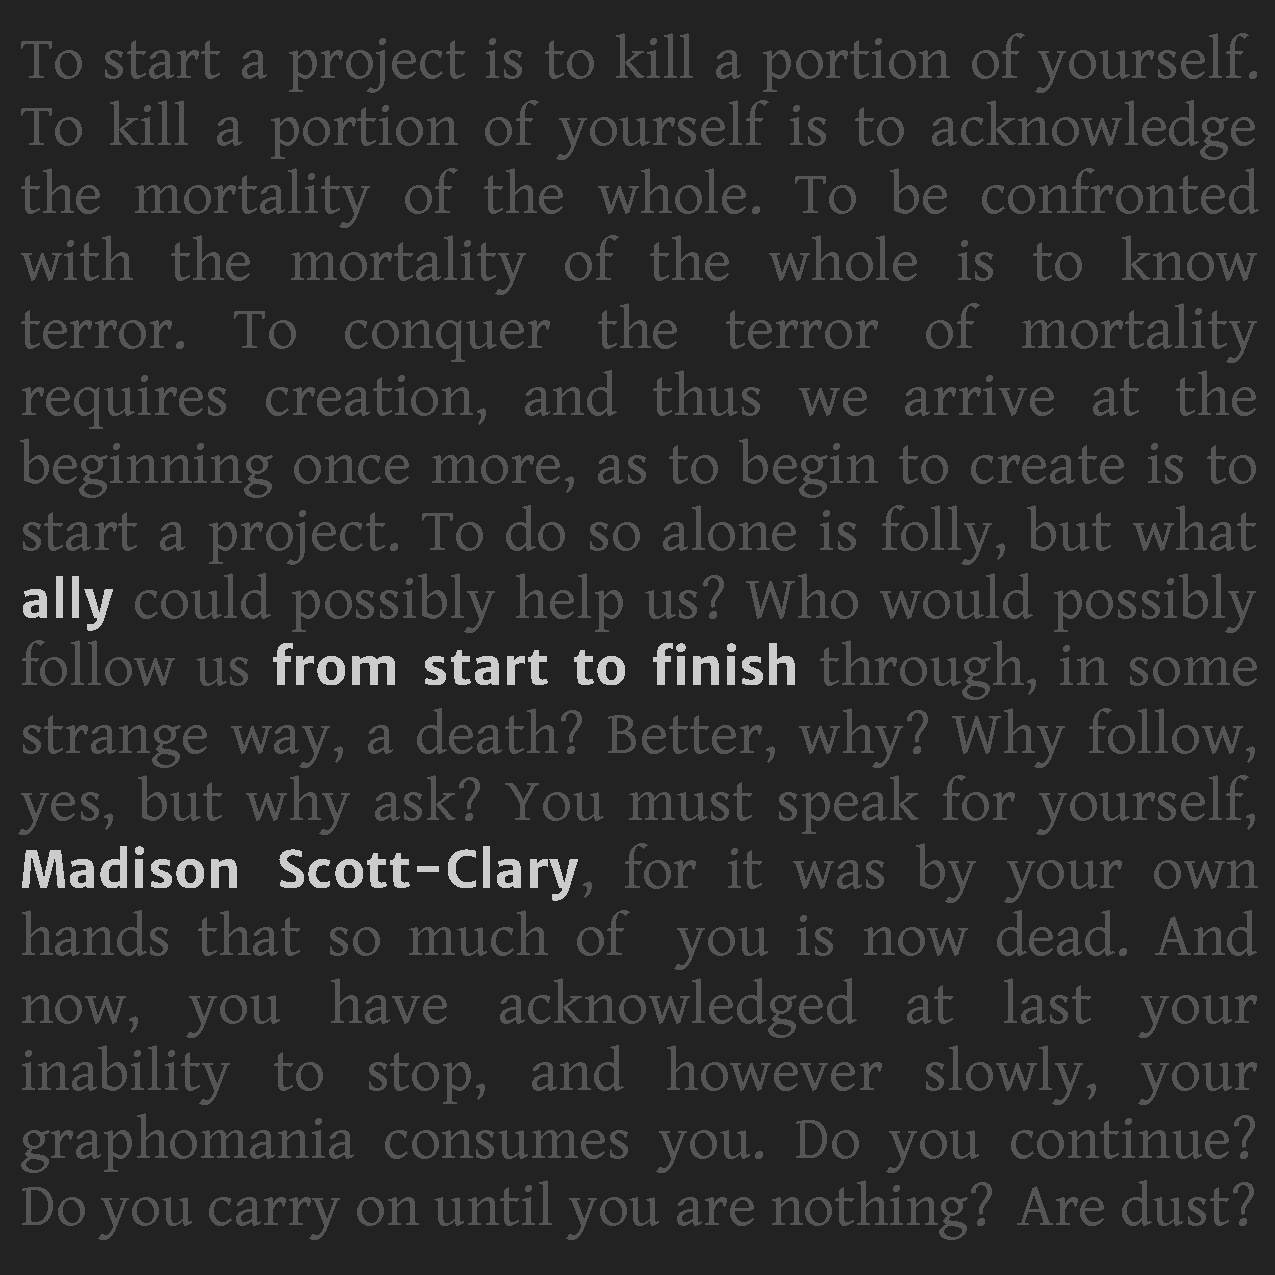
\includepdf{cover.pdf}
  \thispagestyle{empty}
\null
\vfill
\begin{center}
  \FullTitle
\end{center}
\vfill
\cleardoublepage


  \pagestyle{plain}

  \doublespacing

  \null
  \vfill
  \begin{flushright}
    {\fontspec{Merriweather Sans}[Scale=1.5,Color=444444FF]\Huge ally}

    \vfill
    
    {\fontspec{Merriweather Sans}[Scale=1.5,Color=555555FF]\normalsize from start to finish}
    \vfill
    {\Huge Madison Scott-Clary}
  \end{flushright}
  % \vfill
  \thispagestyle{empty}

  \newpage

  
\thispagestyle{empty}
\null
\vfill
\begin{center}
    \noindent\textbf{Also by Madison Scott-Clary}

    \emph{Arcana --- A Tarot Anthology}, ed.

    \emph{Rum and Coke --- Three Short Stories from a Furry Convention}

    \emph{Restless Town}

    \emph{Eigengrau --- Poems 2015--2020}
\end{center}
\vfill
\singlespacing
{\small\parindent0pt\parskip5pt
\noindent All works \copyright\ Madison Scott-Clary except where specified otherwise. These works are licensed under the Creative Commons Attribution 4.0 International License. To view a copy of this license, visit \mbox{\emph{creativecommons.org/licenses/by/4.0/}} or send a letter to Creative Commons, PO Box 1866, Mountain View, CA 94042, USA.

This book uses the fonts Gentium Book Basic and  {\allyFont Merriweather Sans} and was typeset with {\usefont{OT1}{cmr}{m}{n}\XeLaTeX}.

\vspace{1ex}

ISBN: \ISBN

\vspace{1ex}

\emph{\Title}

\vspace{1ex}

First Edition, \Year.

\EditionsList
}

\cleardoublepage


  % \tableofcontents*
  \newpage
  \null
  \thispagestyle{empty}
  \cleardoublepage

  \onehalfspacing

  % \input{content/preface}
  \null
  \vfill
  \begin{center}
    How many layers of remove is enough?

    \vfill

    We ask how, because the question of why must ask itself.
  \end{center}
  \vfill

  \mainmatter

  \pagestyle{ourbook}
  \columnratio{0.65}
  \setlength\columnsep{20pt}
  %\twosided
  \backgroundcolor{c[1]}[HTML]{eeddff}
  \backgroundcolor{C[1](0.5\columnsep,10000pt)(10000pt,10000pt)}[HTML]{eeddff}
  \begin{paracol}{2}
\begin{leftcolumn}
\noindent How does one start a project?

\begin{ally}
  With a bang, or with a whimper?
\end{ally}
Very funny.

In all seriousness, though. How? Does one come up with an idea and just\ldots{}what, go? Just start going and when you get to the end, stop? Can everything be, as NaNoWriMo would have it, pantsed? Run by the seat of your pants such that everything is done without planning, and thus nothing is unsurprising to the author?

Or does one plan meticulously? Does one craft an outline of such startling beauty that to finish the project itself feels almost a betrayal?

\begin{ally}
  Which are you guilty of?
\end{ally}
\end{leftcolumn}
\begin{rightcolumn*}
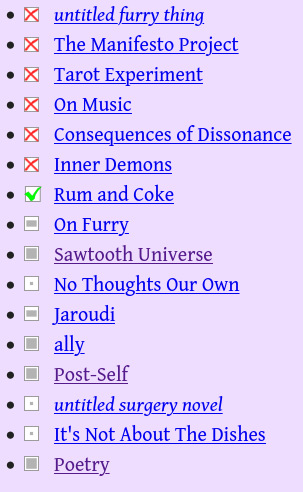
\includegraphics[width=2in]{assets/project-list.png}
\end{rightcolumn*}
\begin{leftcolumn}
Both, of course. I have my fair share of projects I planned so thoroughly that they fell through, just as I have my fair share of projects that I tried worked and worked and worked on and kept adding and adding and adding, and by the end they were so wandery as to be incomprehensible. They didn't hold together, and the story had gone so far off the rails that it was unfixable without a total rewrite.

\begin{ally}
  And which type was I?
\end{ally}
Don't preempt me. All of the projects that I've actually succeeded at have been somewhere in the middle. It's important to plan, as I've learned from all those countless unfinished projects, but there is also a fine balance of planning required, lest you plan your work out of existence.

\emph{Qoheleth}, the book that follows \emph{ally}, has, as a major theme, the difference between honing and forging. To hone is to take an idea and work it to an ever sharper point, whereas to forge is to take an idea, work until its good enough, and forge onwards. 

Neither is bad, of course. There is no value judgement in this distinction. Neither, also, is there any sense of permanence to the label. \emph{ally} was a project borne of forging: I was always trying to do something new with the typography, the wordchoice, the colors and textures of each of the sidequests, and so on. \emph{Restless Town} was a project borne of honing, though. My goal with those stories was to try and somehow come to the finest possible point of the lives involved and the tropes and identities that drive them. I wanted to take aspects of myself --- my gender, my mental health, my sexuality, my polyamory --- and hone each into a story worth reading.

But, as with outlining versus pantsing, one can go too far in either direction.

\begin{ally}
  And still, you will never not giggle when you write `pantsing'.
\end{ally}
Correct.

All that to say that, as Herbert would hvae it, beginnings are such delicate times. To start a project is to kill a portion of yourself, because, whether or not you succeed in finishing the project, whether or not you are trying to hone something to a cruel point or to forge into new territory, you will never start that project again. You will never again be the you who started that project.

\newpage

\begin{ally}
  And so why am I here?
\end{ally}
May I throw your words back at you?

\begin{ally}
  By all means.
\end{ally}
\emph{``Can an ally disinhabit a mind so easily?''}

\begin{ally}
  A question I remember you being decidedly uncomfortable with.
\end{ally}
Yes.

\begin{ally}
  But why am I here \textbf{now}? Why when we are talking about how this project was made?
\end{ally}
Do you not deserve to be here for such a conversation? I trust that you will have little to say of much of the mechanics, but much to say about the process of research.

\begin{ally}
  I do not doubt you. And yet you began this as a list of neat \LaTeX\ things you learned along the way. How often does one write a \LaTeX\ cookbook with one's imaginary friend?
\end{ally}
I don't know. Probably not often. There is precedent, though, for overused literary devices in technical writing. \texttt{Coy}\footnote{\href{https://metacpan.org/pod/Coy}{Coy module on CPAN}}, anyone? 

\begin{verse}
  Error messages\\
  strewn across my terminal.\\
  A vein starts to throb. 
   
  Their reproof adds the\\
  injury of insult to\\
  the shame of failure. 
   
  When a program dies\\
  what you need is a moment\\
  of serenity. 
\end{verse}

Or perhaps you enjoy foxes as I do:

\noindent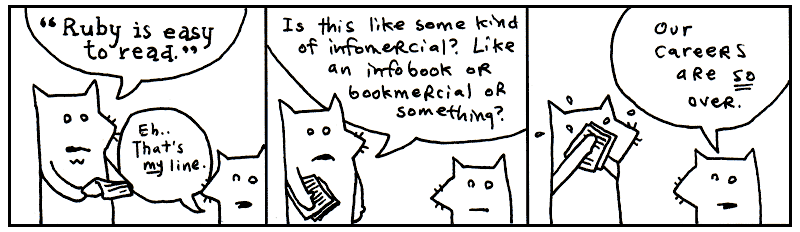
\includegraphics[width=4.2in]{assets/the.foxes-3.png}
\begin{center}
  \footnotesize
  From \href{https://poignant.guide}{\emph{Why's Poignant Guide to Ruby}} by \textbf{Why The Lucky Stiff}, licensed under a CreativeCommons Attribution-ShareAlike license.
\end{center}

There are all sorts of instances of folks writing technical things in a decidedly non-technical fashion.

\begin{ally}
  If you say so. What, then, are you going to talk about in this technical guide?
\end{ally}
Thanks for writing my segue for me.

\begin{labeling}{\textbf{The ally book}}
  \item[\textbf{ally.id}] How the interactive side of ally is built, including some fun examples.

  \emph{Page \pageref{site}}
  \item[\textbf{The ally book}] How the book itself was built.

  \emph{Page \pageref{book}}
  \item[\textbf{Gotchas}] Some problems I ran into along the way.

  \emph{Page \pageref{gotchas}}
\end{labeling}

\end{leftcolumn}
\end{paracol}

  \backgroundcolor{c[1]}[HTML]{ffddee}
  \backgroundcolor{C[1](0.5\columnsep,10000pt)(10000pt,10000pt)}[HTML]{ffddee}
  Everyone, I suspect, deals with movement in a different way. Some are content to sit still where others have to move. Some must move, and it is a part of their personality. Some cannot move and it is a part of their physiology.

And some must move because it is an aching necessity. There is no ``if they do not move, then\ldots{}'' statement to be made. They must move. They can't \emph{not} move.

\begin{quote}
It started as a twitch, you said, as a slight nod of the head.
\end{quote}

Or perhaps it started earlier, I don't know.

\begin{quote}
Perhaps it was all caused by the meds, or perhaps it was presaged by some other restlessness that started years before.
\end{quote}

Perhaps, but does it matter?

\begin{quote}
If it was the meds' fault, you could blame them, but if it was unrelated, you would be able blame yourself. If it was the meds' fault, you could stop, if it was unrelated, you would take that as permission to feel broken.
\end{quote}

Yes, I suppose it does matter, then. That said, I have no answer for that. I just know that it started with a twitch, a slight nod of the head. My fingers would duck up away from the keyboard as though suddenly burned by the keys. I would go and sit in my car over lunch and wring my hands over and over again, occasionally trying to force myself to hold onto the shifter and the door handle, and the tremors would travel up my arms.

Eventually, at some undefinable point, it made its way up into my neck.

I never knew how to explain it.

\begin{quote}
How would you now, with seven years' experience under your belt?
\end{quote}

``Transient tic disorder''. Maybe not so transient before it disappeared, back when I thought it was going to just stick around forever.

\begin{quote}
That's what it's called, but how would you get it across?
\end{quote}

Sobbing? Frustration? Humor? I had a whole comedy set prepared for it, in case I, for some reason, needed to do a stand-up routine.

As you can see, I have a motor tick on my neck that makes me jerk my head to the side and do stuff with my hands. This is because I have transient tic disorder, or as I like to call it, tourettes with holidays.

It makes work life interesting. I stare at a screen all day at my job. Or, well, I stare at my screen and also a point on the wall right about \emph{point} there. It's sort of a timeshare.

I could probably get jobs doing other things, though. Some contract work. Like, hey! Need someone to shake their head `no' at something? I'm your gal. Or maybe you need someone to urgently point something out out with their chin over \emph{point} there. I'd be good at that.

Now, there's a few jobs I won't be good at. Surgeon? Probably not. Bomb squad? That's a definite nope. Professional staring competition participant? I'd be right out. I couldn't win a staring competition with a three year old who's just discovered espresso.

I actually learned about all this tic nonsense at work. It started back in 2012 when it slowly started up over the course of a few days. Went on to find out that it's made worse by stress \emph{lean to the side} stand-up, of course, being the least stressful of occupations \emph{lean back} But no, I worked in health insurance. Health insurance in America as Obamacare is kicking in? Yeah, not exactly a stress-free environment.

Now, this is mostly a motor tic. I don't have the verbal tics that folks associate with tourettes. However, it does make me stutter when it gets bad. If you've never stuttered before,I can tell you that it's infuriating, so, honestly, I didn't need a verbal tic to get me cussing all the time.

So there's me sitting in meetings with other insurance companies, shaking my head `no' to everything they say, and when I try to correct myself, it comes out ``I mean ye-yes FUCK sorry''. I got really good at the whole FUCK-sorry combo.

And so on.

\begin{quote}
How effective do you think that would be on those conference calls with Lewis as you were stuttering away?
\end{quote}

I don't think I could manage. At that point, it was embarrassing enough to have picked up a stutter, a movement disorder that I never explained to my boss or the PM. To acknowledge it to the client would have been mortifying.

  \backgroundcolor{c[1]}[HTML]{ddffee}
  \backgroundcolor{C[1](0.5\columnsep,10000pt)(10000pt,10000pt)}[HTML]{ddffee}
  When I was interviewing for Canonical, the tic had not yet started, or at least not yet to the point where it was affecting my neck or my voice. By the time I \emph{did} start at Canonical, it was well underway.

Much to my chagrin, not only was I stuttering at the time, but the job required daily video calls.

\begin{quote}
You begged off the first few, putting the blame on hardware failures. After the third day, Gary gently suggested that you consider fixing the hardware issues so that the team even knew what you looked like.
\end{quote}

It was embarrassing. Hangouts couldn't even keep up with it. The video was jittery and blurred, my face only in focus for maybe half of the time.

And then, within a few days, it cleared up and went away.

\begin{quote}
The stress of the previous job, of interviewing and those last two weeks, all suddenly relieved in one fell swoop.
\end{quote}

Yes.

\begin{quote}
And then it came back.
\end{quote}

As we all worked from home, the company had us get together in one location four or five times a year for a week at a time in order to work face-to-face and accomplish far more than we would otherwise. They called them sprints, an apt enough comparison.

Copenhagen, though, was different. It was a cascading set of stressors that culminated in, yes, the tic coming back. Two weeks long, with the first half being the developer summit, followed by a week of sprinting. The core product being rewritten. Zephyr getting attacked by another dog while I was away. The hotel, that building \href{/movement/copenhotel.jpg}{canted over to the side at a precarious 15° along two axes}, a nightmare on the acrophobia side.

The tic started up, then got worse and worse.

It was about this time that I started getting closer to Robin, and by the time we had our first real time together at FC 2013, I had shaken my sense of balance from myself and walked with a cane. ``You have a cane,'' she said, part confused, partly out of acknowledgment.

``Yeah, I lost my balance with the tic.''

``That's okay.''

And then we hugged.

\begin{quote}
Not all of it was your balance. Some of it was an apology.
\end{quote}

Yes. Someone with a movement disorder who pretends it isn't there is, in some ineffable way, sadder than someone who at least makes some public acknowledgment that, yes, this is happening. The cane helped. People would see me shaking my head, see me shaky on my feet, and then see the cane and know, ``Ah yes, \emph{this} is happening.''

\begin{quote}
You happened to pass by one of the attendees from the data panel shortly after, and overheard him telling his friend, ``That was a really cool panel, but I think he had Parkinson's or something. Every time he would get more interested in what he was talking about, it would get worse.''
\end{quote}

Yes. Part of me was embarrassed, sure, but part of me was relieved to be seen.

  \label{ally:4}
\begin{paracol}{2}
  \begin{leftcolumn}
\begin{ally}
Why am I here?
\end{ally}
Aren't you always?

\begin{ally}
With you, sure. Why am I bound to words, though? It's been fourteen\index{Numinous!seven} years.
\end{ally}
Surely that's not all on me. You must play some role in it. I was talking with my partner about doing something autobiographical for my next project, after all.

\begin{ally}
I'm the observer and the mirror. All I can do is reflect your choices back at you. Choice itself is not my department.
\end{ally}
After getting \emph{Restless Town}\footnote{makyo.ink/publications/restless-town} finished, I needed something to do. Some other project that would make me feel like I was being productive.

\begin{ally}
Feel, or seem?
\end{ally}
Both. If I sat still, I'd burn up. If I was seen sitting still, clearly I'd be worth less in the eyes of those around me, right?

\begin{ally}
Not my department.\index{ally!Not my department}
\end{ally}
Right.

So I started digging through stuff I'd already done, seeing if any of it could be cleaned up and turned into a new project. I stumbled across \emph{Rum and Coke}\footnote{makyo.ink/publications/rum-and-coke} and found it mostly clean as it was, so I decided to publish it as a book. Paperback and ebook, I mean, not just the stories online.

\begin{ally}
Were you proud of them?
\end{ally}
To an extent. A different me wrote them. A lesser me, in some ways. I was younger, I hadn't quite found my voice and tone. No \emph{Arcana},\footnote{makyo.ink/publications/arcana} no \emph{Disappearance}, no \emph{Getting Lost} or \emph{Post-Self}.\footnote{post-self.github.io} All I had was a few scattered tidbits and my mom's words ringing in my ears: "You wrote your own wedding vows, right? I could tell."

A me with a different identity, too. A me that was working on gender through small steps. I hadn't yet picked up the word 'trans' for myself. I was non-binary, presenting male, writing to justify myself. Or maybe to hype myself up. I was writing works about gender and poly problems being worked through to convince myself it was possible.\index{Gender}

\begin{ally}
They read like parables.
\end{ally}
They were, to me. Each one came with an internal discussion after the last line, \emph{now, what can we take from this?} Something in a circle. Socratic. A talking stick.

\begin{ally}
I know, I was there.
\end{ally}
Of course.

\begin{ally}
Why didn't I show up then?
\end{ally}
I was too\ldots{}something. Too busy, too preoccupied. I was focused too much on identity, too much on The Work, as it were, to reflect. Maybe I was moving too quickly to notice my choices being shown to me.

\begin{ally}
You'd mostly stopped [adjective][species]\footnote{adjectivespecies.com} by\index{Furry![adjective][species]} then, too.
\end{ally}
Life got weird. I was transitioning--

\begin{ally}
A choice.
\end{ally}
--I was solidifying my relationship with Judith--\index{Relationships!Judith}

\begin{ally}
A choice.
\end{ally}
--I was starting to burn out at work--

\begin{ally}
Was that a choice?
\end{ally}
The result of choices, maybe. The result of the choice to start drinking. It \emph{is} called \emph{Rum and Coke}, after all. The result of the choice to get into computers. The result of the choice to work from home, which itself was the result of a choice to take the previous job so far from home.

\begin{ally}
You burned out in part because you burned so hard at the start.
\end{ally}
Was I not supposed to? I had to prove myself.

\begin{ally}
To whom?
\end{ally}
You?

\begin{ally}
Not my department.
\end{ally}
One of your neighbors, perhaps. A cubicle over, a floor above, something like that.

\begin{ally}
Do you anthropomorphize me that much?
\end{ally}
No, I suppose, I don't. You're not my therapist, sitting in a chair across from me and talking me through my problems. You're not person shaped. You're the shape of my hands displaced half an inch behind my own, navy blue and trimmed with sea-foam green.\index{Numinous!colors}

\begin{ally}
You haven't used colors in fourteen years, either.
\end{ally}
What I'm trying to say is that maybe you're back because of nostalgia\index{Nostalgia}. *Restless Town* was done and couldn't be published yet, and a prideful part of me didn't want it to be my first book, so I pulled \emph{Rum and Coke} into shape.

It rubbed my nose in the past. I published it a few weeks ago, and I wasn't done with the past, so I started archiving more data. I dug up my old hard drives. I grabbed stuff from Dreamhost, both files and database backups. I finally unlocked my LJ account and archived that.\index{Nostalgia\index{Nostalgia}}

\begin{ally}
And you work at an archive.
\end{ally}
I go through phases, looking back at the past. I'll spend a few days trying to backdate some log files, or dig through my old scores and publish them --- I did that too, alongside \emph{Rum and Coke}, publish a bunch of my old music --- or resurrect my notes on \emph{Nanon},\footnote{nanon.lang.drab-makyo.com} or the like.

\begin{ally}
You are quite mercurial.
\end{ally}
A failing. That may play a role in my burnout. I'm only good at something for seven years before it becomes so intolerable that I have to leave. Happened with school.

\begin{ally}
So here I am, your ally, twice seven years later.
\end{ally}
I hadn't thought of it that way.

\begin{ally}
Portentous. The only way it would've been more so is if it were thrice seven years.
\end{ally}
I ran away thrice seven years ago. In seventh grade, in 1997, no less.

\begin{ally}
Ill omens. What will happen to me in seven years?
\end{ally}
Will you leave me for good?

\begin{ally}
Can an ally disinhabit a mind so easily?
\end{ally}
I'm not comfortable with that question. I'm not comfortable with its implications. Either way, the past is important to me because maybe it can help me figure out the present. Those who don't know history are doomed to blah blah blah.

\begin{ally}
And have you figured out your present?
\end{ally}
For me to pull out that trite quote about my own personal history speaks pretty well to my fears of doing things accidentally. I've certainly figured out my present better than twice-seven-years-ago me had figured out his.

\newpage
\end{leftcolumn}
\end{paracol}
\index{ally|)}


  %%%%%

  \backmatter
  \pagestyle{empty}

\end{document}
